\section{Methodology}

After laying out the existing research and deriving implications from it, the next step consists of extending these findings. To achieve that a scientific study is in order. How that study is going to be structured is subject of discussion within this chapter. In the following, the research questions are going to be revisited as a starting point for that discussion. For each of the unanswered questions adequate scientific methods to answer them, have to be found. To determine these methods in this chapter, at first additional considerations are laid out. After that, the chosen methodological area(s) is (are) described in more detail. The reasoning and final selection of methods are presented subsequently. Finally, the data generated through the chosen methods has to be analyzed. The way in which this is done is illustrated at the end of this chapter.

\subsection{Methodological Considerations}

To choose the right methods for the research questions at hand, additional considerations have to be taken into account. These considerations consist of the nature of the question (is it an exploratory question, do we want to measure effectiveness, \ldots) and the goal of these questions. The first research question \textbf{(RQ1)} is, \textit{How and which theories \& concepts from research on play can be used in the onboarding process of software development projects and how are developers experiencing them?}. As this is the main research question it is not going to be answered using a single method but rather through collectively answering the other questions and condensing the results.

The second research question \textbf{(RQ2)} is \textit{Which playful themes could lend themselves well to evolve software development projects into spaces of play?}. These strategies, patterns, systems, and theories can also be described as implications for those spaces. The foundation for these design implications was discovered in chapter 2.4. That foundation is expanded upon in the following chapter, where design implications based on literature are fomrulated. The question of which of the implications are effective in onboarding processes is out of scope for this thesis though, as the focus lies in exploring possible implications to start with. Nonetheless, initial, qualitative feedback on a subset of implications that could be implemented should be gathered.

For the third research question \textbf{(RQ3)} -- \textit{What are the technical, social, and personal intricacies of an onboarding context in software development, and how do they influence the onboarding experience?} -- much of the research has already been done. Similar to RQ2, the intricacies of the process were described through researching related literature on exactly this topic. Additional qualitative data should be gathered to answer RQ2 within the upcoming study. It is not the goal, however, to develop generalizable statements about the process. The overall goal is an exploratory one and therefore participant feedback is only used for the argumentation of the qualitative results.

In contrast to RQ2 and RQ3 for the fourth research question \textbf{(RQ4)} -- \textit{How can the identified themes be applied in actual onboarding settings?}, as well as the fifth research question \textbf{(RQ5)} -- \textit{How do different kinds of software developers experience playful aspects within an onboarding context?} -- there is no existing body of work to rely on. Therefore the upcoming study should aim to provide an answer to those two questions in specific and gather additional data for the aspects mentioned concerning RQ2 and RQ3.

To discover adequate methods, RQ4 has to be deconstructed to uncover what exactly should be researched. There are two parts of the question that help with this. Firstly, the notion of \textit{applied} and secondly the phrase \textit{in actual onboarding settings}. Applied strongly points to the practical creation of something that incorporates the implications identified before. A possible approach for this could be to pick a single implication, implement it and then extensively test it with study participants. This could allow for generalizable results for this specific approach, where one could create reproducible results. While such an approach could deliver valuable insights, the downside is its narrow focus on one implementation detail. Another approach could be to implement and maybe even combine multiple implications in one design and gather data on the participants' subjective experience towards them -- which would be the goal of RQ5. The design process of such an approach could also provide data on possible applications for multiple implementations, which in turn allows for a broader answer to RQ4. The downside of researching multiple implementations at the same time is the possible blending of effects of multiple implications. This means that no definitive answer on the effectiveness of one specific implication can be given. On the other hand, it allows for participant feedback on multiple design implications, based on which future research can be done on promising aspects.

As one can see, there is no \enquote{silver bullet approach}, there rather are considerations to make on which approach provides more of the desired results. For this thesis, these are -- as already mentioned more than once before -- very much focused on taking a step into uncharted territory and explore different paths within that. Thus, exploratory, open-ended results are what is aimed for here, which makes for an easier weighting of the arguments presented. This means in the following methods are considered that can provide exactly that.

The second part of RQ4 (\textit{actual onboarding settings}) narrows down options for methods further. As an important aspect of this thesis is the combination of play with the context -- the aforementioned \textit{actual onboarding settings} -- investigating design implications within this context is necessary. This shows the need for a method where the implementation of the design implications can be deployed in the context.

A methodological area that could provide this is \textit{\gls{rtd}}, where through a design (e.g., the implementation of identified implications) research can be done. Important to note here is the need for additional data to provide explorative and personal results. To identify if \gls{rtd} as a whole and its specific methods, in particular, can deliver that, a more detailed description is given in the subsequent chapters. The chosen methods are then laid out in particular, as well as the chosen analysis methods.

\subsection{Research through Design}

To gain a clear picture of what \gls{rtd} is, it is important to understand the differences between design and research as a whole. Fortunately, Stolterman describes these differences very well. Research, or more specifically scientific research, he explains, drives towards the existing and universal knowledge. Specifically, Stolterman mentions that \enquote{The aim of science is to formulate universal knowledge that explains the complexities of reality on a level removed from specifics and particulars} \cite[p. 57]{stolterman2008nature}.

On the other hand, \enquote{design deals with the specific, intentional and non-existing} \cite[p. 59]{stolterman2008nature}. Certainly, this kind of research has proven very useful to generate \enquote{knowledge about natural objects and phenomena} \cite[p. 3]{simon2019sciences}. Research on and with man-made \textit{artificial} objects asks for a different science, as Simon has argued even dating back to the late 1960s \cite{simon2019sciences}. Simon also further defined aspects of a science of design, describing designers as, everyone who \enquote{devises courses of action aimed at changing existing situations into preferred ones} \cite[p. 111]{simon2019sciences}. This notion of creating preferred futures generally prevailed. Coughlan et al. specifically mentioned designing prototypes as a way to create such futures and contrasts it to the traditional science approach:

\begin{quote}
  \textit{In its essence as a design synthesis tool, prototyping represents commitment to a new future. In contrast, prolonged analysis of existing or historical practices (implicit in many of the articles in this issue), even though undertaken with the goal of future change, inevitably feels rearward facing}

  \footnotesize{Coughlan et al. \cite[p. 132]{coughlan2007prototypes}}
\end{quote}

As already mentioned before, this aligns with the goal of the thesis overall -- to branch out into the future, to create new ways of how to onboard software developers. In addition to that, there is a need to research a multitude of applied implications. Overall, this suggests a designerly approach being the right methodological choice here. Critics might argue that such an approach is missing rigor and reproducibility. While especially the aspect of reproducibility cannot be denied, it has to be said, that \enquote{Design research conducted according to strict scientific procedures can produce highly valuable knowledge} \cite[p. 60]{stolterman2008nature}. To create this valuable knowledge, a strict scientific procedure has to be selected. This is where \gls{rtd} comes into play. The term was first coined by Sir Christopher Frayling \cite{frayling1994research} and brought into the field of \gls{hci} by Zimmerman et al. \cite{zimmerman2007research}. They describe \gls{rtd} in \gls{hci} as a way to produce novel integrations of research into HCI to create something that represents the preferred state of the world \cite[p. 493]{zimmerman2007research}.

\gls{rtd} as a whole can be described more broadly as a way to conduct scholarly research with methods originating from design practice \cite{zimmerman2014research} \enquote{as a legitimate method of inquiry} \cite[p. 310]{zimmerman2010analysis}. Zimmerman et al. also reinforce the arguments on why \gls{rtd} would be an adequate methodology in the case of this thesis:

\begin{quote}
  \textit{RtD allows researchers to rely on designerly activities as a way of approaching messy situations with unclear or even conflicting agendas; situations that are not well suited to other methods of inquiry. Additionally, RtD forces researchers to focus on research of the future, instead of on the present or the past.}

  \footnotesize{Zimmerman et al. \cite[p. 310]{zimmerman2010analysis}}
\end{quote}

Zimmerman also proposes criteria for evaluating \gls{rtd} approaches to ensure that as much scientific rigor as possible is applied to such approaches. The four criteria proposed are:

\begin{itemize}
  \item{\textbf{Process} -- \enquote{In documenting their contributions, interaction design researchers must provide enough detail that the process they employed can be reproduced. In addition, they must provide a rationale for their selection of the specific methods they employed} \cite[p. 499]{zimmerman2007research}}
  \item{\textbf{Invention} -- \enquote{The [...] contribution must constitute a significant invention [...] researchers must demonstrate that they have produced a novel integration of various subject matters to address a specific situation} \cite[p. 499]{zimmerman2007research}}
  \item{\textbf{Relevance} -- \enquote{researchers must also articulate the preferred state their design attempts to achieve and provide support for why the community should consider this state to be preferred} \cite[p. 499-500]{zimmerman2007research}}
  \item{\textbf{Extensibility} -- \enquote{defined as the ability to build on the resulting outcomes of the interaction design research: either employing the process in a future design problem, or understanding and leveraging the knowledge created by the resulting artifacts} \cite[p. 500]{zimmerman2007research}}
\end{itemize}

Delivering on all those aspects is crucial in order to allow for valuable knowledge generation despite not following a traditional research approach. Therefore, these criteria are going to be referred back to throughout both the study and the results of this thesis, starting with the process. Creating such a process from scratch could weaken the study's results, as an unproven approach has to be validated in itself (independently from the results of its application). Thus, following and documenting a proven process as part of a proven set of methods is necessary here. Within \gls{rtd} a multitude of different methods emerged since its integration into \gls{hci}. Fortunately, Sanders condensed years of research on design research as a whole and condensed it into a map of said design research, as visible in \textit{Figure \ref{fig:researchtypes}}.

\begin{figure}[h]
  \centering
  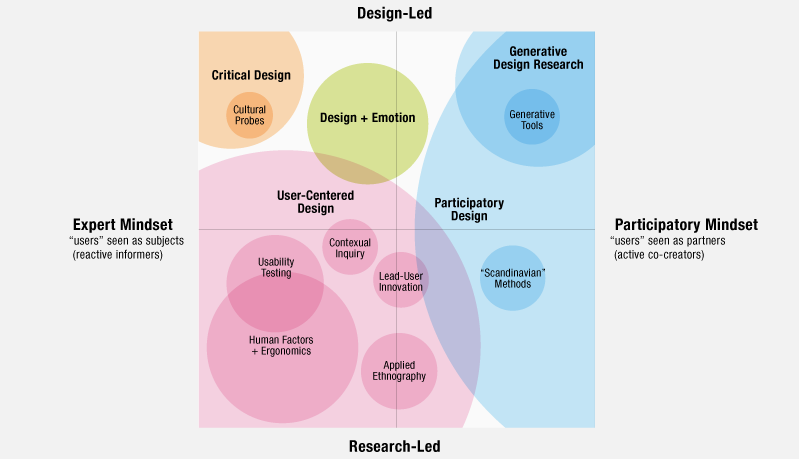
\includegraphics[width=0.9\textwidth]{researchtypes}
  \caption{\enquote{Map of design research -- research types} by Liz Sanders \cite[p. 3]{sanders2008evolving}}
  \label{fig:researchtypes}
\end{figure}

It is important to note here, that this does not show a map of \gls{rtd} methods specifically, but a more complete one of many methods applied in \gls{hci}. The two axis of the map describe firstly, which research type the methods align to -- either design-led or research-led, based on the distinction described earlier. Secondly, the so-called \textit{mindset} focuses on if an expert creates something that then is relayed to the users or if the users are active co-creators as Sanders puts it \cite[p. 5-6]{sanders2008evolving}. \gls{rtd} can be located mainly in the upper-left quadrant of this map, although it can be argued that some methods include the user as a more active part. Generally, though, \gls{rtd} is based upon careful preparation by experts and therefore gravitates towards the aforementioned expert mindset. In \textit{Figure \ref{fig:researchtypes-probes}} Sanders extended her original map with some more methods.

\begin{figure}[h]
  \centering
  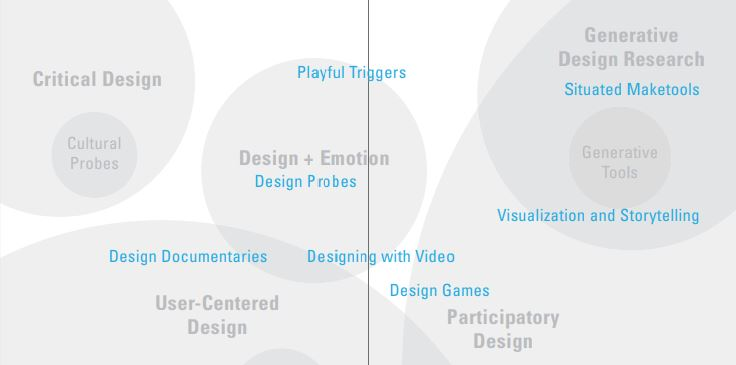
\includegraphics[width=0.7\textwidth]{researchtypes-probes}
  \caption{Upper section: \enquote{Map of design research -- new tools and methods} by Liz Sanders \cite[p. 6]{sanders2008evolving}}
  \label{fig:researchtypes-probes}
\end{figure}

To narrow down the methodological choices it is crucial to estimate where this study would fall within the presented map. Concerning the research-led vs. design-led, the case has already been made for a distinctly design-led approach. Regarding the mindset, the answer is a bit less obvious. While we do want to gather information directly from developers in actual onboarding settings, this does not necessarily mean that they are participating in the design process itself. Most of the work on the theoretical foundation design is already done, therefore at that step, there is a need for additional input. Where additional input \textit{is} needed, is at the transition from implemented implications towards recommendations and starting points for future research. An approach where both the expert mindset and partly active participation is possible would thus be the desired one. On the map methods allowing for this would subsequently be located in the middle of the upper section.

In that section we can find the two methods \textit{Playful Triggers} and \textit{Design Probes}. The term \textit{playful} strongly suggests that this might be the right method to research play. Upon closer inspection, it might not be fully applicable to this study, though, as \enquote{This methodology utilises playful, tactile, everyday qualities of objects} \cite[p. 16]{akama2010community} that then \enquote{take on the meanings placed on them by the participants} \cite[p. 16]{akama2010community} to facilitate conversation. This would align with the goal of researching how developers experience (and how open they are towards) such playful triggers in onboarding processes, but disregards the implementation part of the study. In addition to that tangible interaction together with facilitated on-site collaboration is hard to execute due to ongoing work-from-home mandates due to the COVID-19 pandemic. Therefore, it is required that the chosen method can be executed remotely. A closer look into \textit{Design Probes} consequently is the next step. As these exist in many variations, these have to be discussed in order to choose a suitable of these variations.

\subsection{Probing in a Digital Context}

Before delving into these variations, the origin of probing has to be mentioned, as it is going to help in understanding the process and goals of what came after. This origin can easily be traced back to Gaver et al., who first mentioned \textit{Cultural Probes} as a research method in 1999 \cite{gaver1999design}. Gaver et al. were tasked with researching novel interaction techniques for the elderly within their local communities. The difficulty they were faced with, was the cultural difference between them (the experts) and elderly from different parts of Europe. To overcome these difficulties, they developed these so-called cultural probes, \enquote{packages of maps, postcards, and other materials [...] designed to provoke inspirational responses from elderly people in diverse communities} \cite[p. 22]{gaver1999design}. According to Gaver et al. these probes \enquote{address a common dilemma in developing projects for unfamiliar groups} \cite[p. 22]{gaver1999design}. The aforementioned parts of the probes (postcards, maps and more) were designed to be approached casually and to spark open-ended discussion. The probes consisted of two other parts as well. Firstly, questions were included, that concerned the environment of the elderly. These were as open-ended as possible in order to give the participants as much room as possible to answer casually. Secondly, the probes included a self-documenting aspect. Participants were tasked to take record specific actions daily for a week \cite[p. 22-26]{gaver1999design}. Concerning the particular goals, Gaver et al. also mention gaining \enquote{new understandings of technology} \cite[p. 25]{gaver1999design} and designing to \enquote{shift current perceptions of technology functionally, aesthetically, culturally, and even politically} \cite[p. 25]{gaver1999design}. Another important aspect is that the resulting data is not guided by a single problem statement, instead it is inspirational data that is collected throughout the process. The actual launch of the probes was then done in meetings at the local sites, after which the participants used the probes to self-document as described earlier. Finally, Gaver et al. also describe how, even though \enquote{the probes were central to our understanding of the sites, they didn’t directly lead to our designs} \cite[p. 29]{gaver1999design}. Cultural probes are widely used nowadays in \gls{hci} research \cite{crabtree2003designing,wyeth2006designing,kjeldskov2004using,celikoglu2017user,fisher2016adapting}. So widely used in fact that multiple variations developed from these cultural probes.

One that is particularly interesting in the context of researching digital artifacts are \textit{technology probes}. This term was coined by Hutchinson et al., who originally used it as a way to design technologies for and with families \cite{hutchinson2003technology}. They deployed two different technology probes in two different contexts, a \textit{VideoProbe} and a \textit{MessageProbe}. Independent from these different probes, what Hutchinson et al. wanted to achieve was to gain knowledge and user feedback early on in the design process. Not only that, they wanted \enquote{them to be active partners in the design process} \cite[p. 2]{hutchinson2003technology}. It has to be noted, that Hutchinson et al. did not go so far as to \enquote{expect the family members to become designers} \cite[p. 18]{hutchinson2003technology}. What is also mentioned is where exactly these \textit{technology probes} differ from \textit{cultural probes}, \enquote{cultural probes tend to involve a single activity at a particular time and do not stress technology per se} \cite[p. 18]{hutchinson2003technology}. Thus, the ultimate goal of a \textit{technology probe} is similar to that of traditional \textit{cultural probes}, albeit more focused on a specific technology -- \enquote{Ideally, technology probes will spark new ideas and help the families articulate ideas for the prototypes we will build} \cite[p. 18]{hutchinson2003technology}. To create a \textit{technology probe} that can achieve such a goal, Hutchinson et al. define the five following features:

\begin{itemize}
  \item{\textbf{Functionality} -- \enquote{Technology probes should be as simple as possible, usually with a single main purpose and two or three easily accessible functions} \cite[p. 18]{hutchinson2003technology}}
  \item{\textbf{Usability} -- \enquote{Technology probes are not primarily about usability in the HCI sense, so during the use period, we do not change functions} \cite[p. 18]{hutchinson2003technology}}
  \item{\textbf{Logging} -- \enquote{Technology probes collect data about relationships within the family and help family members (and us) generate ideas for new technology} \cite[p. 18]{hutchinson2003technology}}
  \item{\textbf{Flexibility} -- \enquote{technology probes [...] should be designed to be open-ended with respect to use} \cite[p. 19]{hutchinson2003technology}}
  \item{\textbf{Design Phase} -- \enquote{Technology probes are intended to be introduced early in the design process as a tool for challenging pre-existing ideas and influencing future design} \cite[p. 19]{hutchinson2003technology}}
\end{itemize}

These would be the criteria, a possible technological implementation in the upcoming study strives for. This stands in contrast to a prototype, that is much more feature-rich from the beginning, focuses on usability and is improved iteratively (rather than implementing something new based on the data gathered through a probe) \cite[p. 18-19]{hutchinson2003technology}. Generally speaking one could describe these technology probes as a middle ground between cultural probes and the evaluation and implementation of full-blown prototypes. This is also in contrast to so-called \textit{digital cultural probes}, as e.g., Iversen \& Nielsen applied it \cite{iversen2003using}. They went for more of a traditional approach with a stark focus on self-documentation and content generated by the participants, rather than deploying an implementation for them to use.

At this point, the question arises on what to take from all of that regarding the methodological decision at hand. Answering that question requires contrasting the research goals with what probes in general and \textit{technology probes} in particular provide. The overall goal of the thesis is to explore new opportunities for playful approaches in an onboarding context as mentioned numerous times before. Thus, there is a need for a method that at its core is exploratory. Probes certainly can provide that, as Mattelmäki describes in her doctoral thesis on \textit{Design Probes} as a whole. She writes that \enquote{probes have an exploratory character. They explore new opportunities rather than solve problems that are known already} \cite[p. 40]{mattelmaki2006design}.

Another important point mentioned mainly in RQ5 is the need to research how software developers experience playful aspects. Researching this could arguably be the biggest strength of probing. Mattelmäki describes it as follows, \enquote{probes look at the user’s personal context and perceptions. The purpose is to outline human phenomena and users, as well as introduce the user’s perspective to enrich design} \cite[p. 40]{mattelmaki2006design}. This is also described by Gaver et al. as \enquote{The real strength of the method was that we had designed and produced the materials specifically for this project, for those people, and for their environments} \cite[p. 29]{gaver1999design}. \textit{Technology probes} in particular can provide even more value in the case of this thesis. RQ4 and RQ5 also call for testing out implementations of the design implications in real-world settings, while still being open towards new input from developers. Referring back to Hutchinson et al., they describe the goals of \textit{technology probes} as:

\begin{quote}
  \textit{the social science goal of collecting data about the use of the technology in a real-world setting, the engineering goal of field-testing the technology, and the design goal of inspiring users and designers to think about new technologies}

  \footnotesize{Hutchinson et al. \cite[p. 17]{hutchinson2003technology}}
\end{quote}

This, again, closely aligns with the research goals of this thesis -- there is a need for collecting data on the design implications in \textit{actual onboarding settings}. There is also a need to \textit{field-test} these digitally implemented implications. Finally, there is also -- as mentioned before -- a need to still be open about new input, enriching what was discovered in literature. Overall, the alignment of goals points towards \textit{technology probes} as the method of choice for the study. The relatively good adoption of this method (e.g. in \cite{fitton2004probing,o2006holding,edwards2011exploring}) further manifests it as an adequate choice.

At this point, the only thing left is to define a rough overall process for the execution of this method. That process is then elaborated on in great detail in chapter 4 to ensure the study manages to meet the quality criteria for a well done \gls{rtd} approach, as described by Zimmerman \cite[p. 499]{zimmerman2007research}. It is crucial to mention some environmental constraints to the study here. Firstly, we are working with digital source code with which the participants (software developers) have to (mostly) interact with in a digital environment. Secondly, as acknowledged before, as of June 2021, many software developers are choosing or being ordered to work from home due to the COVID-19 pandemic. Therefore, it is necessary that the chosen process can be executed remotely.

There is no single process to follow when designing, executing, and analyzing \textit{probes}. Gaver et al. even mentioned that the \enquote{probes were not designed to be analyzed, nor did we summarize what they revealed about the sites as an explicit stage in the process} \cite[p. 27]{gaver1999design}. Hutchinson et al. on the other hand mentioned \textit{logging} and analyzing interactions as a distinct part of the process. How this is done, differs from study to study. Edwards et al. for example, logged user-generated data and created accompanying questionnaires to collect quantitative data on the use of their probes \cite[p. 107-110]{edwards2011exploring}. Mattelmäki proposes personal interviews to \enquote{extend, supplement and revise the signals collected in the probes} \cite[p. 86]{mattelmaki2006design} where qualitative data is generated. Ultimately, there is great variance in the execution as well as the analysis of these probes. This makes it even more important to carefully lay out every part of the final process.

Overall, there are three distinct areas that are part of the process, the development \& implementation of the probes, their execution \& deployment, and the analysis of the data generated through the probes. Concerning the development of the probes, the path is pretty clear, as the features within the probe should be based on the identified design implications. The specific process of how these were transformed into probe features is described in great detail in chapters 4.2 and 4.2.1.

After the \textit{technology probe} is developed it then has to be deployed into the context and executed by the participants. Therein it is important to gather the data needed to answer the research questions. Thus, generating data on personal experiences, as well as exploratory data is paramount. This strongly suggests collecting qualitative data, as it is uniquely able to gather perspectives of participants \cite[p. 7-8]{flick2018introduction} as well as generating new knowledge on a setting too pluralized for quantitative approaches \cite[p. 4-5]{flick2018introduction}.

That does not mean there is no structured data at all, though. As \textit{logging} is such an integral part of \textit{technology probes}, user interactions with the features of the probe are going to be logged. To get an even more complete understanding of how the individual participants experienced the probe and to gather qualitative input on new ideas from participants, qualitative questions are going to be asked after probe execution. Additionally, to get a sense of how effective the probe features were, in actually transmitting information about a project, questions on the project at hand are asked as well. This allows for a rich set of data for each participant to analyze. The focus strongly lies in generating as much valuable data as possible for each participant rather than aiming for a maximum number of participants. Overall there is going to be a three-step process concerning the probes:

\begin{enumerate}
  \item{Probe Development}
  \item{Probe Execution \& Data Collection}
  \item{Probe Analysis}
\end{enumerate}

As mentioned, the specific tasks within these steps are going to be described in great detail with every additional process choice documented as well in chapter 4. Concerning the probe analysis, the methods of analyzing the generated data is subject of the following chapter.

\subsection{Data Analysis}

The last high-level methodological choice to make is concerned with how to analyze the data gathered by the probing. To recapitulate, data is going to be gathered through these four methods:

\begin{itemize}
  \item{\textbf{Demographic Information} -- Prior to the probes some information on the professional background of the participants is gathered to gain a comprehensive picture of the participants}
  \item{\textbf{Participant Interactions} -- Throughout the probe the actions taken by the participants are going to be logged and categorized in an automated way (e.g. a click on an element on the screen)}
  \item{\textbf{Questions on the underlying project} -- The participants are going to be asked questions on the project they are onboarded on to}
  \item{\textbf{Questions on the research topic} -- The participants are going to be asked questions centered around the research topic to gather their expertise and ideas on the topic}
\end{itemize}

In order to correctly analyze that data, it is crucial to know what kind of data is generated by each of these. Only after that a suitable method of analysis can be found.

To start of the demographic information consists of a set of fixed data types (e.g., age always equals a number). These do not have to be analyzed on their own, they rather set the data in an individual context for each of the participants.

The interactions on the other hand are going to be automatically logged during the study. Therefore, the logs need to follow a predefined structure so that a variety of different interactions can be persisted. The actual structure of these interactions is described in chapter 4.3 as it also depends on the technology used to capture these events. These interactions could for example be analyzed in a way to find patterns of interactions, like analyzing the number of clicks at a certain point in time. This might be very useful to delve into specific aspects of the probe and analyze them in great detail (see Fitton et al. for example \cite{fitton2004probing}). While this can be useful for intricate features, these are not really the part of the probe, as it should be kept simple. In addition to that evaluating the effectiveness and details of these particular features is not the prime goal of this study. Nonetheless, it can help in solidifying arguments based on the other kinds of data and can be referred to together with participant feedback. Because of that the interactions together with the time of each interaction is going to be logged but only analyzed in detail as needed. Simple aggregations of total interactions and total time spent within the probe are generated from the raw logs, though, to give a sense of how active the in-probe interaction was.

Moving on to the questions on the underlying project, these should help in understanding how the participants experienced the probe. The goal of these questions should be to understand if the underlying information was transported successfully. The questions should be crafted in a way, that allows for verifying if the participants recognized the project information. Lastly, the arguably most important part is to gather data on the experiences of the participants, their attitude towards playfulness in onboarding processes, and their ideas on how to integrate it. As already described in the previous chapter a qualitative approach was chosen for that. Concerning the actual creation of the questions, these are centered around the specific topic at hand, similar to how problem-centered interviews are structured around an issue \cite{witzel2012problem}.

The actual data collection for these problem-centered interviews revolves mainly around in-person inquiries, mirroring and lively discussion \cite[p. 232-236]{flick2018introduction}. Due to the study being a remote one, such a lively discussion might be hard to execute. Therefore online interviewing, as mentioned by Flick \cite[p. 243]{flick2018introduction} could be a more adequate solution.

This type of interviewing can be done in a few different ways. Probably, the two most important decisions concerning the study design are, if the questions should be answered asynchronously or synchronously, and through which medium the questions are asked. This largely depends on the study setup, as it could be possible to integrate the questions within the probe or the medium over which the probe is interacted with. Thus, the rationale for this decision is described in the subsequent chapter. This final decision does not change the method to analyze the data, as this data consists of unstructured text that is going to be used for qualitative argumentation.

Depending on the amount of data gathered, there are different options for analysis. From using the participant feedback directly, to applying a specific method of analysis, there is a broad range of possibilities. On the more rigorous end of the scale, two of the most notable approaches are thematical analysis \cite{braun2006using} and content analysis \cite{schreier2012qualitative}. These mainly differ in how they develop themes and categories, where themes are generated from text (thematical analysis) or text is analyzed with a set of categories in mind (content analysis) \cite[p. 490]{flick2018introduction}. Concerning the research done within this thesis, a lot of themes and implications were already discovered, therefore it might make a lot of sense to use them as a starting point for the analysis. This should make content analysis a suitable choice for analyzing the data. Executing it involves multiple steps, as described by Schreier and Flick (\cite[p. 174]{schreier2014ways}, \cite[p. 483-485]{flick2018introduction}:

\begin{enumerate}
  \item{Selection of the material}
  \item{Creation of a category system}
  \item{Segmentation of the material}
  \item{Main coding}
  \item{Interpretation and Presentation}
\end{enumerate}

Within those steps, additional methodological decisions and considerations have to be made. Concerning the first step, selection is trivial. As the study is specifically crafted to generate qualitative data, all the qualitative answers within that study are subject to analysis. Thus, all answers by each participant on the research topic and the underlying project are selected for the content analysis. The additional data collected throughout the probe is used as a support for the result argumentation, as was mentioned before.

Regarding step two, the creation of a category scheme, there are three distinct options of coming up with these categories -- \textit{Deductive, Inductive and Deductive-Inductive}. The decision on one of these approaches mainly depends on if the result argumentation should be derived from the material (inductive) or defined by literature and brought to the material (deductive). Mixed approaches exist as well, where some categories are brought to the material and some are based on the material (deductive-inductive), for example by defining top-level categories from literature and lower-level categories from literature for example \cite{schreier2014ways}.

This is what is going to be done in the case of this study, with the overall direction of the analysis defined through the literature and the research questions, while also allowing for new categories and themes based on text.

Concerning step three, a unit of segmentation has to be defined. Two options -- that can again be mixed and inform each other -- are coding units and contextual units. Coding units carry meaning by themselves and can be definitively allocated to a category, while contextual units help in giving meaning to the coding units \cite{schreier2014ways}.

In the context of this study, the material is divided into coding units. Where necessary or helpful to give context, contextual units are used. These contextual units can either be the features/questions they refer to, but also the logged data, where it supports the argumentation.

The coding itself is then done as a two-step process, with marking important units at first and then coding these marked units in a second step, as described by Schreier \cite{schreier2014ways}. The interpretation and presentation ultimately can be found in detail in chapter 5.2 and onwards.